\section{Introduction}\label{sec:Intro}
Micro- and nano-robots can be manufactured in large numbers.
Our vision is for large swarms of robots remotely guided 1) through the human body, to cure disease, heal tissue, and prevent infection and 2) ex vivo to assemble structures in parallel. 
 For each application, large numbers of micro robots are required  to deliver sufficient payloads, but the small size of these robots makes it difficult to perform onboard computation.  Instead, these robots are often controlled by a global, broadcast signal. 
 Future implementations require control techniques that can reliably exploit large populations despite significant under-actuation.  
 

\begin{figure}
\begin{center}
	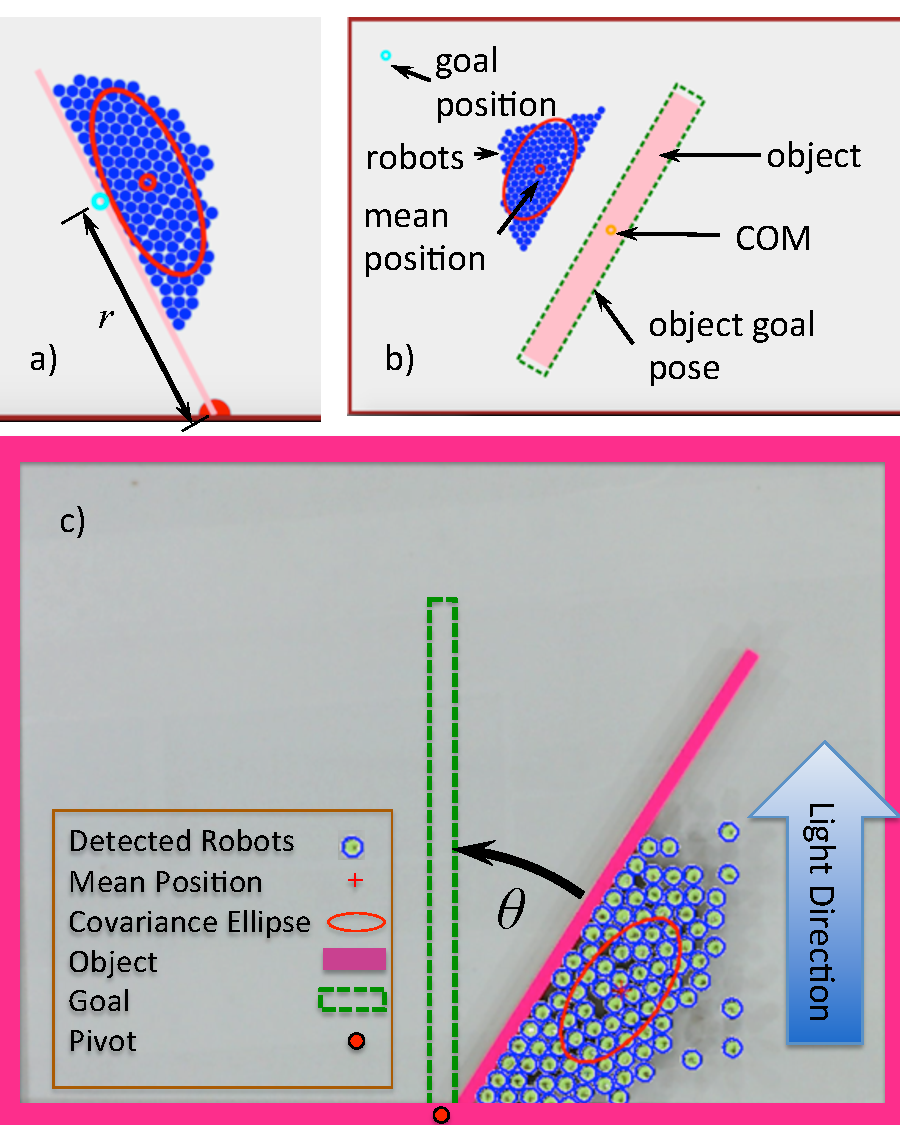
\includegraphics[width=.9\columnwidth]{CoverPhoto.pdf}
\end{center}
\vspace{-1em}
\caption{\label{fig:FirstImage}
Torque control of an object is essential for manipulating objects to their goal position  when there are narrow passageways and for aligning sensors, emitters, or other objects. 
This paper provides feedback control laws to apply torques and forces using a highly under-actuated system where all 
robots are controlled globally by the same input. 
(a) Simulation of robots exerting torque on a hinged ``door''.
(b) Simulation of swarm orientation manipulation.
(c) 97 hardware robots applying torque to an object. These robots have light sensors and are programmed to move toward the brightest light in the room.  This light is a shared control input that operates globally on the swarm.
}
\vspace{-1em}
\end{figure}


%One surprising result was that humans that only knew the swarm's mean and covariance completed the task faster that humans who knew the position of every robot~\cite{Becker2013b}. Our previous work focused on a block-pushing task, where a swarm of robots pushed a larger block through a 2D maze. 
Previous work proved that the mean position of a swarm is controllable and that, with an obstacle, the swarm's position variance orthogonal to rectangular boundary walls  is also controllable
(these are $\sigma_x$ and $\sigma_y$ for a workspace with axis-aligned walls). 
The usefulness of these techniques was demonstrated by several automatic controllers. One controller steered a swarm of robots to push a larger block through a 2D maze~\cite{ShahrokhiIROS2015}. 
We also showed methods to control a swarm's position covariance to enable navigating the swarm through a workspaces with narrow corridors.  
However, object manipulation often also requires controlling torque on an object, for example changing the orientation of an object with a large aspect ratio to thread through narrow corridors.
Torque control  is also necessary for a variety of alignment tasks from retroreflectors, mirrors for solar incinerators, to targeted radiation therapy.

Accurate torque control is difficult.
A swarm with $n$ agents has $2n$ degrees of freedom.  
This swarm, when steered toward an object, begins interacting with object at different times. 
The number of robots touching this object as a function of time is difficult to predict and often impossible to directly measure.
Stochastic effects make long-term prediction challenging.
Even when it is possible to predict which agents will hit the object first, as agents interact with the object, the swarm's configuration changes.
The challenge is not only limited to swarm-object interaction, but also to swarm-swarm interactions when the swarm self-collides  or is split into multiple components. 
As a result, the force the swarm will exert on the object is not easy to predict.
Predicting the force a swarm exerts on an object requires knowing the location of every robot in contact with the object. 
This information is often hard to gather, because remote sensing of tiny particles is difficult.
Particles may be smaller than the minimum resolution of MRI, PET, and ultrasound, but these sensing modalities can still return aggregate data.
From this aggregate data,  some statistics---including mean and variance---are easy to obtain. 
Rather than design open-loop algorithms, this paper focuses on feedback control strategies using just two statistics of the swarm, the mean and variance of the swarm's position. Fig. 1 illustrates the torque control using 97 kilobots, as well as two simulation snapshots of torque and orientation control (Section \ref{sec:simulation} and Section \ref{sec:expResults}).

%This paper first discusses the ways that we can control torque of an object in Section ~\ref{sec:theory}. Then it introduces algorithms for torque control in Section ~\ref{sec:simulation}. We show that algorithms work in Section ~\ref{sec:expResults} on 100 kilobots.

%For controlling $\sigma_{xy}$, we prove that the swarm position covariance $\sigma_{xy}$ is controllable given boundaries with non-zero friction. 
%We then prove that two orthogonal boundaries with high friction are sufficient to arbitrarily position a swarm of $n$ robots. 
%We conclude by designing controllers that efficiently regulate $\sigma_{xy}$.


%This paper
%(1) proves that the swarm position covariance $\sigma_{xy}$ is controllable given boundaries with non-zero friction,  %where do we do this?
%(2) proves that two orthogonal boundaries with high friction are sufficient to arbitrarily position two robots, 
%(3) proves that two orthogonal boundaries with high friction are sufficient to arbitrarily position a swarm of $n$ robots, 
%(4) shows full-state position control with 2 or more robots using  extensive simulations, and
%(5) demonstrate covariance control on our hardware platform with a large number of hardware robots.
%TODO JOURNAL: design controllers that efficiently regulate $\sigma_{xy}$.
%TODO JOURNAL: We will design Lyapunov-inspired controllers for $\sigma_{xy}$ to prove controllability. 
%TODO JOURNAL:  and rank controllability as a function of friction.
% TODO: JOURNAL: and vary wall friction by laser-cutting boundary walls with a variety of profiles. 







% Our paper is organized as follows.  After a discussion of related work in Section \ref{sec:RelatedWork}, we describe our experimental methods for an online human-user experiment in Section \ref{sec:expMethods}.  We report the results of our experiments in Section \ref{sec:expResults}, discuss the lessons learned in Section \ref{sec:discussion}, and end with concluding remarks in Section \ref{sec:conclusion}.


